\begin{figure}[t]
\centering
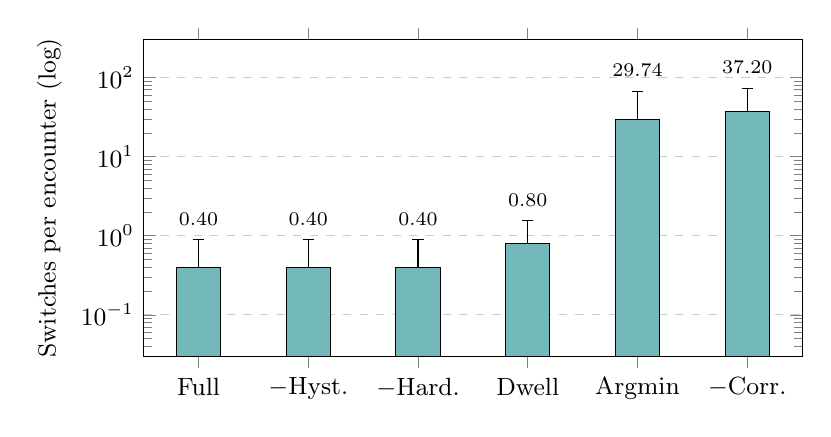
\begin{tikzpicture}
\begin{axis}[
  width=0.82\linewidth, height=5.6cm,
  ybar, bar width=16pt, ymode=log, log origin=infty,
  ymin=0.03, ymax=300,
  xtick={0,...,5}, xticklabels={{Full},{$-$Hyst.},{$-$Hard.},{Dwell},{Argmin},{$-$Corr.}},
  ylabel={Switches per encounter (log)},
  ymajorgrids, grid style={dashed,gray!40},
  error bars/y dir=plus, error bars/y explicit,
  enlarge x limits=0.1, tick label style={font=\small}, label style={font=\small},
]
\addplot[fill=teal!55, draw=black, error bars/.cd, y dir=plus, y explicit] coordinates {
(0,0.4000) +- (0,0.4909)
(1,0.4000) +- (0,0.4909)
(2,0.4000) +- (0,0.4909)
(3,0.8000) +- (0,0.7498)
(4,29.7440) +- (0,36.7008)
(5,37.2000) +- (0,36.1198)
};
\node[font=\scriptsize,anchor=south] at (axis cs:0,1.0245) {0.40};
\node[font=\scriptsize,anchor=south] at (axis cs:1,1.0245) {0.40};
\node[font=\scriptsize,anchor=south] at (axis cs:2,1.0245) {0.40};
\node[font=\scriptsize,anchor=south] at (axis cs:3,1.7823) {0.80};
\node[font=\scriptsize,anchor=south] at (axis cs:4,76.4115) {29.74};
\node[font=\scriptsize,anchor=south] at (axis cs:5,84.3178) {37.20};
\end{axis}
\end{tikzpicture}
\caption{\textbf{Class-switch count per encounter by variant} (mean with $+$SD whisker, log scale; $N=250$ per variant, 5 scenarios $\times$ 50 seeds, 10.0~s horizon), regenerated with pgfplots from \texttt{ablation\_raw.csv}. The immediate-argmin policy and the synthetic correspondence-loss stress comparator ($-$Corr.) yield 29.74 and 37.20 decision changes per encounter, respectively, whereas the proposed method (Full) maintains commitment with 0.40. Removing hysteresis ($-$Hyst.) or progress hardening ($-$Hard.) alone shows no observed regression in this scenario set, supporting the accumulator configuration's suppression of fluctuations in this scenario set; the synthetic comparator does not identify the causal effect of correspondence.}
\label{fig:oscillation}
\end{figure}
